\section{Исследовательский раздел}
\subsection{Условия исследований}
Исследование проводилось на персональном вычислительной машине со следующими характеристиками:

\begin{itemize}
\item процессор Apple M1 Pro,
\item операционная система Ventura 13.5.2,
\item 32 Гб оперативной памяти.
\end{itemize}

\subsection{Визуализация графа}

На рисунке \ref{img:1} представлена визуализация графа без использования средств построения макета.

\begin{figure}[H]
	\centering
	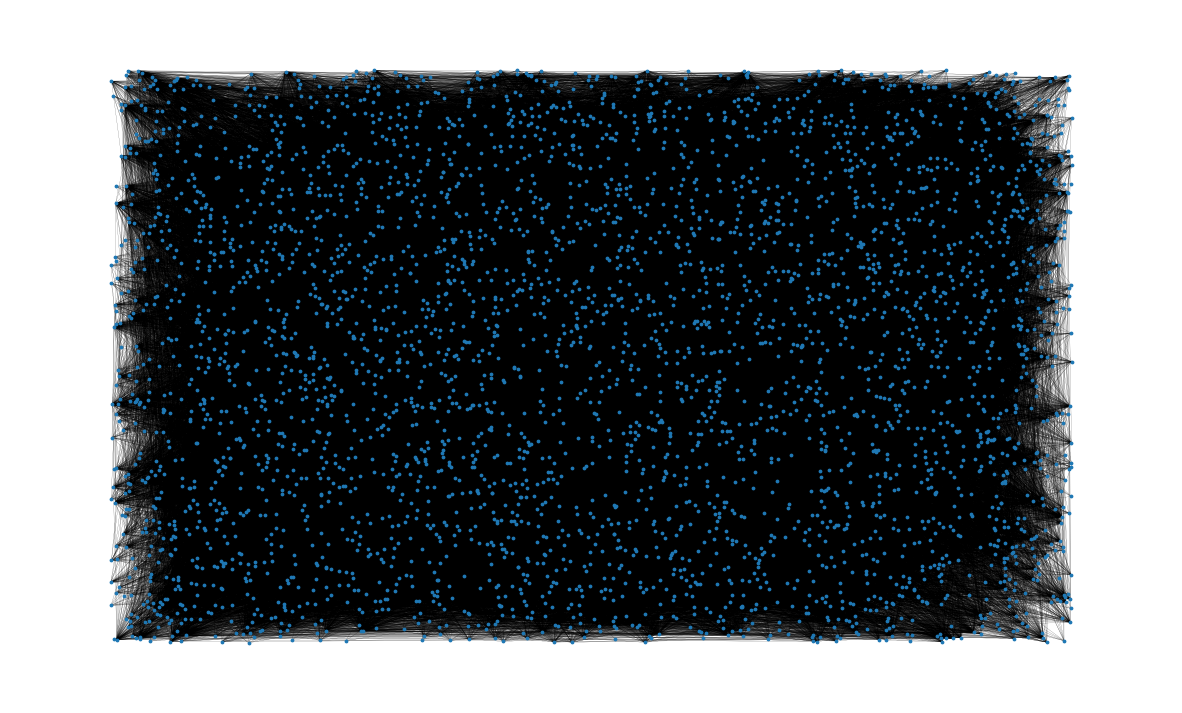
\includegraphics[width=\textwidth]{inc/1.png}
	\caption{ Визуализация графа.}
	\label{img:1}
\end{figure}

На рисунках \ref{img:2} -- \ref{img:4} представлена визуализация графа с использованием функции построения макета \textbf{spring layout} при количестве итераций 15, 30 и 50 соответственно.

\begin{figure}[H]
	\centering
	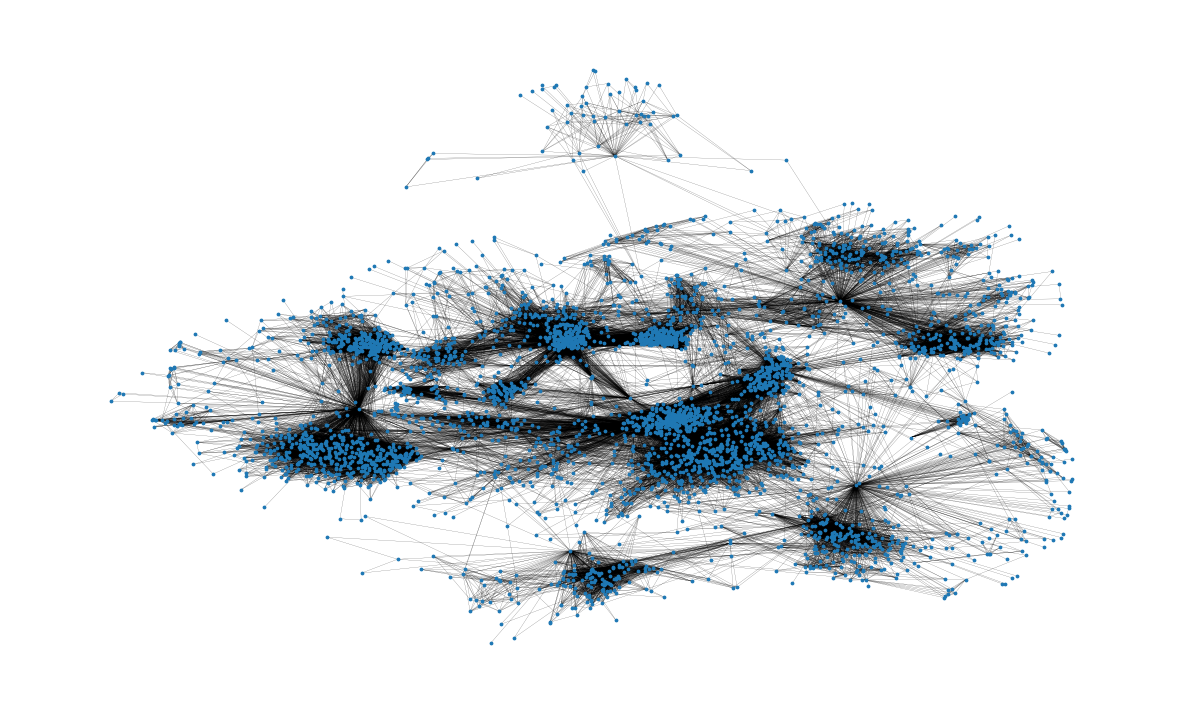
\includegraphics[width=\textwidth]{inc/2.png}
	\caption{ Визуализация графа с использованием функции \textbf{spring layout}, количество итераций 15.}
	\label{img:2}
\end{figure}

\begin{figure}[H]
	\centering
	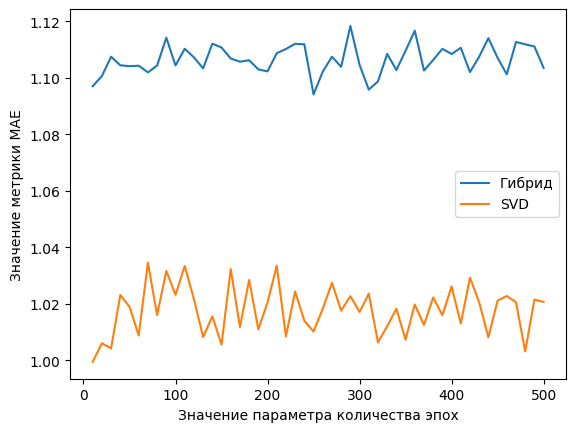
\includegraphics[width=\textwidth]{inc/3.png}
	\caption{ Визуализация графа с использованием функции \textbf{spring layout}, количество итераций 30.}
	\label{img:3}
\end{figure}

\begin{figure}[H]
	\centering
	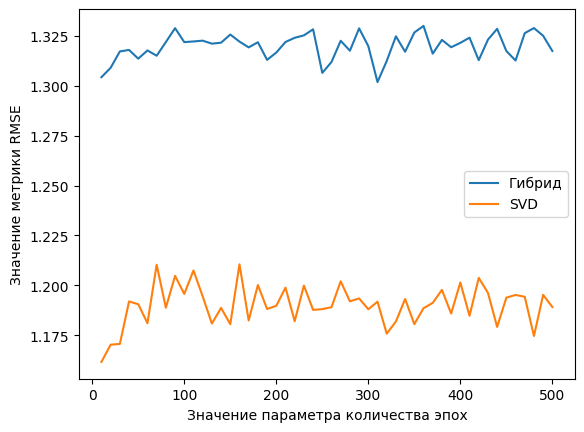
\includegraphics[width=\textwidth]{inc/4.png}
	\caption{ Визуализация графа с использованием функции \textbf{spring layout}, количество итераций 50.}
	\label{img:4}
\end{figure}

В качестве используемого при визуализации результатов работы алгоритмов обнаружения сообществ будет использоваться граф, визуализированный при количестве итераций 50.

\subsection{Результаты работы алгоритмов}

На рисунке \ref{img:5} представлен результат работы алгоритма Label Propogation Communities. Всего было выделено 73 сообщества. В текущей визуализации сложно сказать, что алгоритм однозначно хорошо справился со своей задачей, однако он обнаружил малые сообщества, которые мы уже не увидим в следующих алгоритмах.

\begin{figure}[H]
	\centering
	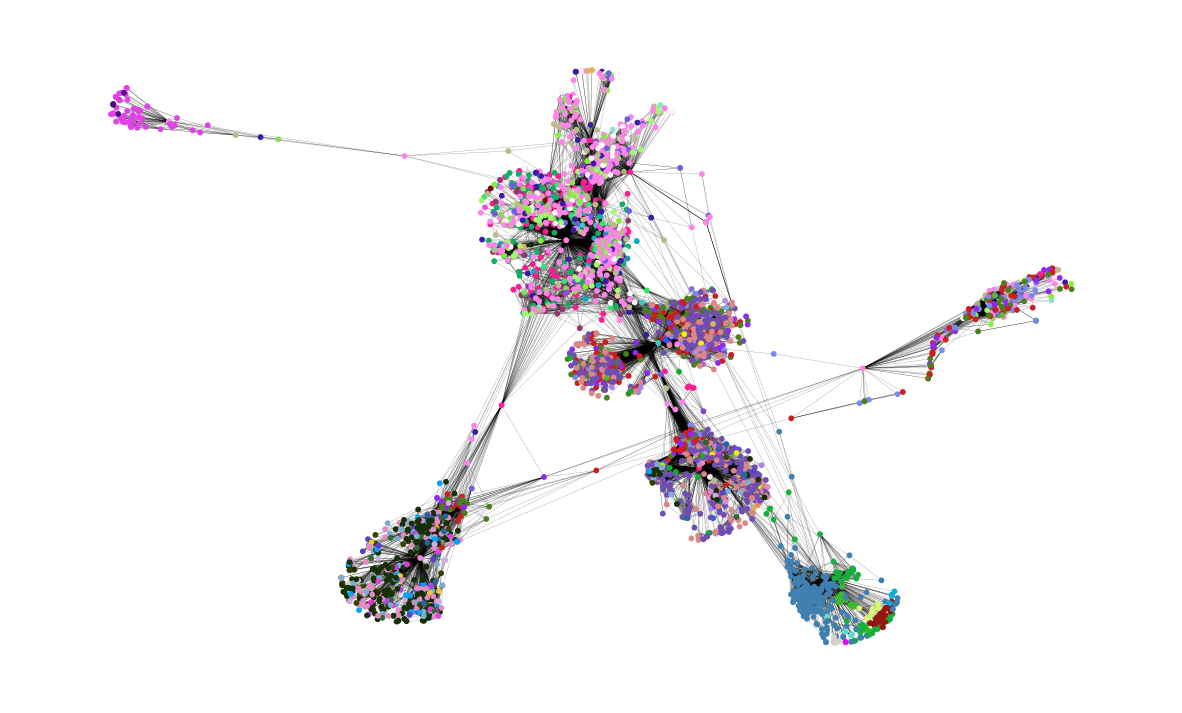
\includegraphics[width=\textwidth]{inc/5.png}
	\caption{ Визуализация результата работы алгоритма Label Propogation Communities.}
	\label{img:5}
\end{figure}

На рисунке \ref{img:6} представлен результат работы алгоритма Лювина. Всего было выявлено 16 сообществ. Алгоритм неплохо справился с поставленной задачей, явно можно увидеть 3 выделенных сообщества, а также 4 области с пересекающимися интересами.

\begin{figure}[H]
	\centering
	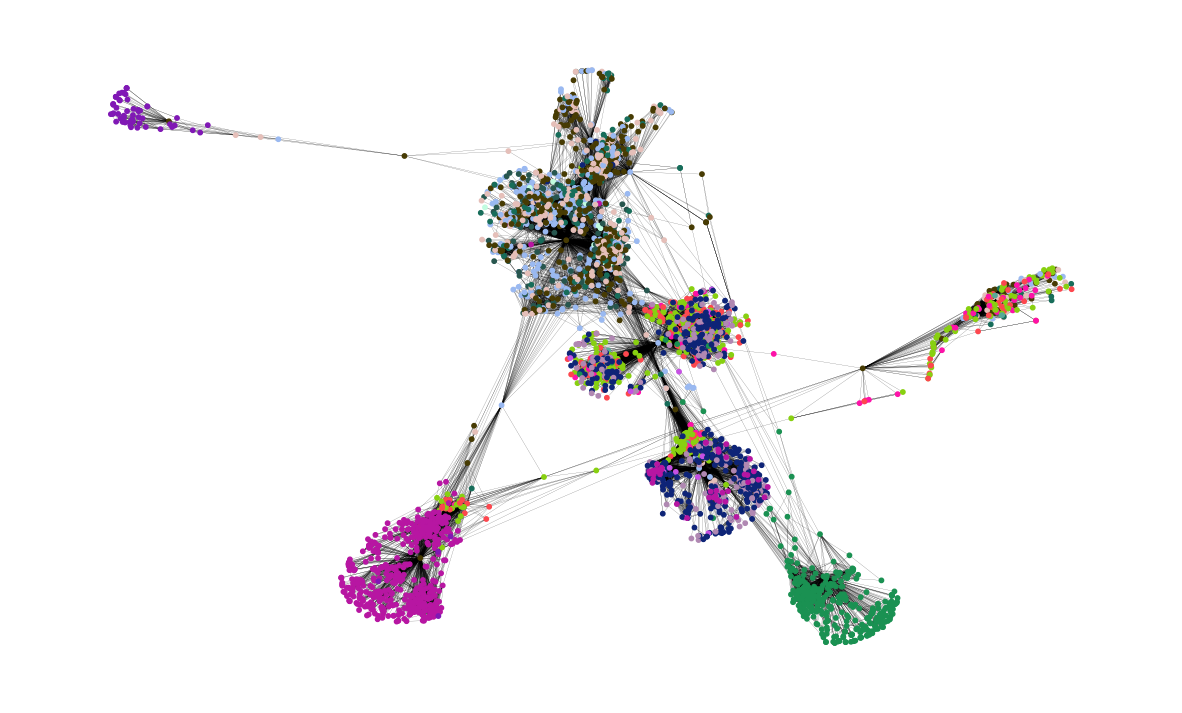
\includegraphics[width=\textwidth]{inc/6.png}
	\caption{ Визуализация результата работы алгоритма Лювина.}
	\label{img:6}
\end{figure}

На рисунке \ref{img:7} представлен результат работы алгоритма Fluid Communities. Заданное количество сообществ 16.


\begin{figure}[H]
	\centering
	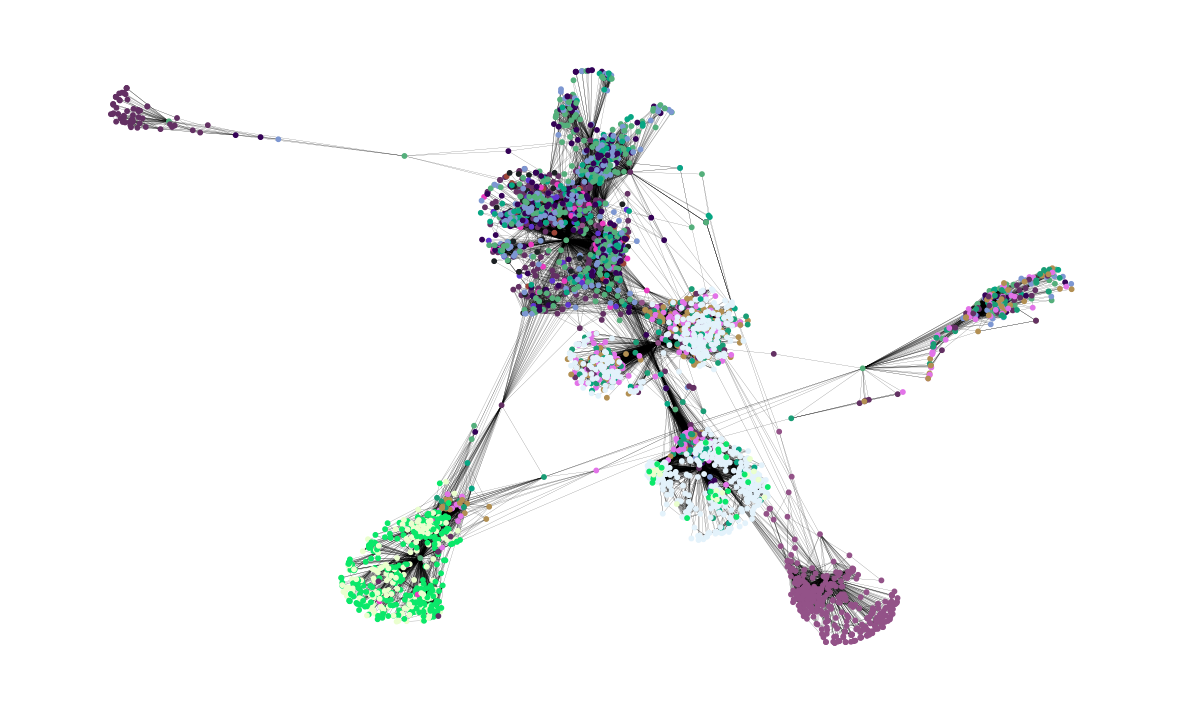
\includegraphics[width=\textwidth]{inc/7.png}
	\caption{ Визуализация результата работы алгоритма Fluid Communities.}
	\label{img:7}
\end{figure}

\subsection{Зависимость времени исполнения алгоритмов от количества связей в графе}

На рисунке \ref{img:8} представлена зависимость времени исполнения алгоритмов LPC, Лювина и Fluid Communities от количества связей в графе.

\begin{figure}[H]
	\centering
	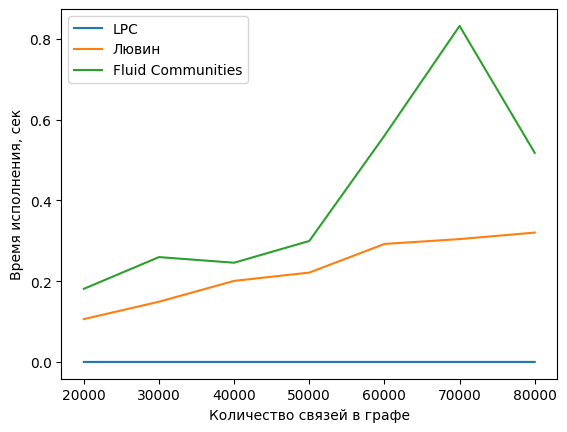
\includegraphics[width=\textwidth]{inc/8.png}
	\caption{ Зависимость времени исполнения алгоритмов от количества связей в графе.}
	\label{img:8}
\end{figure}

\subsection*{Заключение}

В результате проведенных исследований, было получено представление о методах визуализации графов.

Приведенные зависимости времени исполнения алгоритмов от количества связей в графе показало, что даже на достаточно небольшом графе в 80000 связей алгоритмы Лювина и Fluid Communities уже могут исполняться более $0.2$ секунд. Кроме того, легко увидеть, что алгоритм Fluid Communities, несмотря на собственное асинхронное исполнение, однозначно проигрывает по времени исполнения и алгоритму Лювина и алгоритму LPC. Кроме того, из графика видно, что алгоритм LPC выполняется на несколько порядков быстрее двух остальных алгоритмов.